\documentclass[11pt]{article}

\usepackage{latexsym}
\usepackage{graphicx}
\usepackage{amssymb}
\usepackage{amsthm}
\usepackage{enumerate}
\usepackage{amsmath}
\usepackage{cancel}
\numberwithin{equation}{section}

\setlength{\evensidemargin}{.25in}
\setlength{\oddsidemargin}{-.25in}
\setlength{\topmargin}{-.75in}
\setlength{\textwidth}{6.5in}
\setlength{\textheight}{9.5in}
\newcommand{\due}{March 3rd, 2010}
\newcommand{\HWnum}{7}
\newcommand{\grad}{\bold\nabla}
\newcommand{\vecE}{\vec{E}}
\newcommand{\scrptR}{\vec{\mathfrak{R}}}
\newcommand{\kapa}{\frac{1}{4\pi\epsilon_0}}
\newcommand{\expt}[1]{\langle{#1}\rangle}

\begin{document}
\begin{titlepage}
\setlength{\topmargin}{1.5in}
\begin{center}
\Huge{Physics 3320} \\
\LARGE{Principles of Electricity and Magnetism II} \\
\Large{Professor Ana Maria Rey} \\[1cm]

\huge{Homework \#\HWnum}\\[0.5cm]

\large{Joe Becker} \\
\large{SID: 810-07-1484} \\
\large{\due} 

\end{center}

\end{titlepage}



\section{Problem \#1}
\begin{enumerate}[(a)]
\item
In the classical sense the particle is initially moving at a kinetic energy of $E$. Where $E$ is given by
$$E = \frac{1}{2}mv_i^2$$
where $v_i$ is the initial velocity of the particle. But at the step at $x=0$ the kinetic energy of the particle increases to $E+V_0$. So we can say that
$$E+V_0 = \frac{1}{2}mv_f^2$$
where $v_f$ is the final velocity. So if we solve for $v_f$ we get
\begin{align*}
\frac{1}{2}mv_f^2 &= E+V_0\\
\frac{1}{2}mv_f^2 &= \frac{1}{2}mv_i^2+V_0\\
v_f^2 &= v_i^2+\frac{2V_0}{m}\\
v_f &= \sqrt{v_i^2+\frac{2V_0}{m}}
\end{align*}

\item
Given the \emph{Time-Independent Schr\"{o}dinger equation}
\begin{equation}
-\frac{\hbar^2}{2m}\frac{d^2\psi}{dx^2}+V\psi = E\psi 
\label{TISE}
\end{equation}
we can see that the potential in each region is constant and in the left region we see that $V=0$ so for this region we can solve equation \ref{TISE} as
\begin{align*}
-\frac{\hbar^2}{2m}\frac{d^2\psi}{dx^2}+\cancelto{0}{V\psi} &= E\psi\\
\frac{d^2\psi}{dx^2} &= -\frac{2mE}{\hbar^2}\psi
\end{align*}
Now if we guess that the solution is
$$\psi(x) = e^{kx}$$
we see that 
\begin{align*}
\frac{d^2\psi}{dx^2} &= -\frac{2mE}{\hbar^2}\psi\\
k^2e^{kx} &= -\frac{2mE}{\hbar^2}e^{kx}\\
k &= \sqrt{-\frac{2mE}{\hbar^2}}
\end{align*}
So we can say that our general solution to equation \ref{TISE} is
$$\psi_{I}(x) = Ae^{ikx}+Be^{-ikx}$$
note that we have two linearly independent solutions. Where $A$ and $B$ are found using initial conditions. And $k$ is given by
$$k\equiv\frac{\sqrt{2mE}}{\hbar}$$
Now for the right region where $V=-V_0$ we see that equation \ref{TISE} becomes
\begin{align*}
-\frac{\hbar^2}{2m}\frac{d^2\psi}{dx^2}-V_0\psi &= E\psi\\
-\frac{\hbar^2}{2m}\frac{d^2\psi}{dx^2} &= (E+V_0)\psi\\
\frac{d^2\psi}{dx^2} &= -\frac{2m(E+V_0)}{\hbar^2}\psi
\end{align*}
Again if we guess 
$$\psi = e^{kx}$$
we get
\begin{align*}
\frac{d^2\psi}{dx^2} &= -\frac{2m(E+V_0)}{\hbar^2}\psi\\
k^2e^{kx} &= -\frac{2m(E+V_0)}{\hbar^2}e^{kx}\\
k &= \sqrt{-\frac{2m(E+V_0)}{\hbar^2}}
\end{align*}
So we can say the general solution is given by
$$\psi_{II}(x) = Ce^{ik'x}+De^{-ik'x}$$
where 
$$k'\equiv\frac{\sqrt{2m(E+V_0)}}{\hbar}$$
Now we can apply boundary conditions. We can see that from construction we do not have any left moving particles in the right region. This implies that the left moving solution's pre-factor is zero or that $D=0$ so 
$$\psi_{II}(x) = Ce^{ik'x}$$ 
We also know that $\psi(x)$ and $\psi'(x)$ have to be continuous everywhere. This implies the boundary conditions
$$\psi_I(0) = \psi_{II}(0)$$
and 
$$\psi_I'(0) = \psi_{II}'(0)$$
So if we can say that
\begin{align*}
\psi_I(0) &= \psi_{II}(0)\\
Ae^{ik0}+Be^{-ik0} &= Ce^{ik'0}\\
A+B &= C
\end{align*}
And the other boundary condition yields 
\begin{align*}
\psi_I'(0) &= \psi_{II}'(0)\\
Ake^{ik0}-Bke^{-ik0} &= Ck'e^{ik'0}\\
iAk-iBk &= iCk'\\
Ak-Bk &= Ak'+Bk'\\
A(k-k') &= B(k+k')\\
B &= \frac{k-k'}{k+k'}A
\end{align*}
Note that we have $B$ in terms of $A$ and we can find $C$ in terms of $A$ by saying
\begin{align*}
A+B &= C\\
A+\frac{k-k'}{k+k'}A &= C\\
C &= A\left(1+\frac{k-k'}{k+k'}\right)
\end{align*}
So our full solution for $\psi$ is given by
\begin{align*}
\psi(x) &= \psi_I(x)+\psi_{II}(x)\\
&= Ae^{ikx}+Be^{-ikx}+Ce^{ik'x}\\
&= Ae^{ikx}+A\frac{k-k'}{k+k'}e^{-ikx}+A\left(1+\frac{k-k'}{k+k'}\right)e^{ik'x}
\end{align*}

\item
Now if we want to find the reflection and transmission coefficients we say that the reflection coefficient is the probability current of the left traveling wave (with the pre-factor $B$) over the incident wave (pre-factor $A$). We can use 
\begin{equation}
J=\frac{\hbar}{m}\Im\left[\psi^*\frac{d}{dx}\psi\right]
\label{ProbCurr}
\end{equation}
to find the probability current so for the incident wave we can find $J$ as
\begin{align*}
J_{inc} &= \frac{\hbar}{m}\Im\left[\psi^*\frac{d}{dx}\psi\right]\\
&= \frac{\hbar}{m}\Im\left[A^*e^{-ikx}Akie^{ikx}\right]\\
&= \frac{\hbar}{m}\Im\left[ik|A|^2\right]\\
&= \frac{\hbar k}{m}|A|^2
\end{align*}
And for the reflected probability current we can say
\begin{align*}
J_{refl} &= \frac{\hbar}{m}\Im\left[\psi^*\frac{d}{dx}\psi\right]\\
&= \frac{\hbar}{m}\Im\left[B^*e^{ikx}\left(-Bkie^{-ikx}\right)\right]\\
&= \frac{\hbar}{m}\Im\left[-ik|B|^2\right]\\
&= -\frac{\hbar k}{m}|B|^2
\end{align*}
And to find the transmission coefficient we need to find the probability current of the transmitted wave
\begin{align*}
J_{tran} &= \frac{\hbar}{m}\Im\left[\psi^*\frac{d}{dx}\psi\right]\\
&= \frac{\hbar}{m}\Im\left[C^*e^{-ik'x}Ck'ie^{ik'x}\right]\\
&= \frac{\hbar}{m}\Im\left[ik'|C|^2\right]\\
&= \frac{\hbar k'}{m}|C|^2
\end{align*}
Now we can find the reflection coefficient, $R$, we say that
\begin{align*}
R &= \frac{-J_{refl}}{J_{inc}}\\
&= \frac{\hbar k}{m}|B|^2\frac{m}{\hbar k}\frac{1}{|A|^2}\\
&= \frac{|B|^2}{|A|^2}\\
&= \left(\frac{k-k'}{k+k'}\right)^2\frac{A^2}{A^2}\\
&= \left(\frac{\sqrt{2mE}-\sqrt{2m(E+V_0)}}{\sqrt{2mE}+\sqrt{2m(E+V_0)}}\right)^2\\
\end{align*}
And to find $T$ we say that
\begin{align*}
T &= \frac{J_{tran}}{J_{inc}}\\
&= \frac{\hbar k'}{m}|C|^2\frac{m}{\hbar k}\frac{1}{|A|^2}\\
&= \frac{k'}{k}\frac{|C|^2}{|A|^2}\\
&= \frac{k'}{k}\left(1+\frac{k-k'}{k+k'}\right)^2\frac{A^2}{A^2}\\
&= \frac{\sqrt{2m(E+V_0)}}{\sqrt{2mE}}\left(1+\frac{\sqrt{2mE}-\sqrt{2m(E+V_0)}}{\sqrt{2mE}+\sqrt{2m(E+V_0)}}\right)^2\\
&= \frac{\sqrt{E+V_0}}{\sqrt{E}}\left(1+\frac{\sqrt{2mE}-\sqrt{2m(E+V_0)}}{\sqrt{2mE}+\sqrt{2m(E+V_0)}}\right)^2\\
\end{align*}
Now if we add $T$ and $R$ we can see that note that we are using $k$ and $k'$ so it looks cleaner and we are saying that 
$$Q\equiv\frac{k-k'}{k+k'}$$
\begin{align*}
T+R &= \frac{k'}{k}\left(1+\frac{k-k'}{k+k'}\right)^2+\left(\frac{k-k'}{k+k'}\right)^2\\
&= \frac{k'}{k}\left(1+Q\right)^2+Q^2\\
&= \frac{k'}{k}\left(1+2Q+Q^2\right)+Q^2\\
&= \frac{k'}{k}\left(1+2\frac{k-k'}{k+k'}+\left(\frac{k-k'}{k+k'}\right)^2\right)+\left(\frac{k-k'}{k+k'}\right)^2\\
&= \frac{k'}{k}\left(1+2\frac{k-k'}{k+k'}+\frac{k^2+k'^2-2kk'}{k^2+k'^2+2kk'}\right)+\frac{k^2+k'^2-2kk'}{k^2+k'^2+2kk'}\\
&= \frac{k'}{k}\left(1+2\frac{(k-k')(k+k')}{k^2+k'^2+2kk'}+\frac{k^2+k'^2-2kk'}{k^2+k'^2+2kk'}\right)+\frac{k^2+k'^2-2kk'}{k^2+k'^2+2kk'}
\end{align*}
\begin{align*}
&= \frac{k'}{k}\left(1+\frac{2k^2-2k'^2+k^2+k'^2-2kk'}{k^2+k'^2+2kk'}\right)+\frac{k^2+k'^2-2kk'}{k^2+k'^2+2kk'}\\
&= \frac{k'}{k}\left(\frac{k^2+k'^2+2kk'}{k^2+k'^2+2kk'}+\frac{3k^2-k'^2-2kk'}{k^2+k'^2+2kk'}\right)+\frac{k^2+k'^2-2kk'}{k^2+k'^2+2kk'}\\
&= \frac{k'}{k}\left(\frac{k^2+k'^2+2kk'+3k^2-k'^2-2kk'}{k^2+k'^2+2kk'}\right)+\frac{k^2+k'^2-2kk'}{k^2+k'^2+2kk'}\\
&= \frac{4k^2k'}{k(k^2+k'^2+2kk')}+\frac{k(k^2+k'^2-2kk')}{k(k^2+k'^2+2kk')}\\
&= \frac{4k^2k'+k^3+kk'^2-2k^2k'}{k(k^2+k'^2+2kk')}\\
&= \frac{2k^2k'+k^3+kk'^2}{k(k^2+k'^2+2kk')}\\
&= \frac{k(2kk'+k^2+k'^2)}{k(k^2+k'^2+2kk')} = 1
\end{align*}
We see that the particle has to be reflected or transmitted, this makes sense or else the particle would be somewhere we couldn't know. The strange thing is that the particle can be reflected where we saw in part (a) that it will always be transmitted.

\item Assumming that $m=1$ and $E=1$\\
\begin{center}
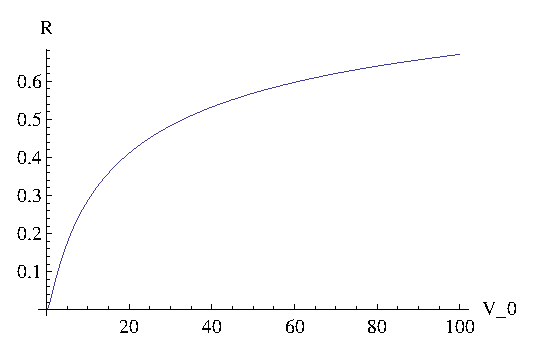
\includegraphics[scale=1.0]{Prob1.partd.eps}
\end{center}


\item
Given that $E=4\ MeV$ and $V_0 = 12\ MeV$ we can see that probability that the neutron will be absorbed is given by the transmission coefficient which we found in part (c) as
\begin{align*}
T &= \frac{\sqrt{E+V_0}}{\sqrt{E}}\left(1+\frac{\sqrt{2mE}-\sqrt{2m(E+V_0)}}{\sqrt{2mE}+\sqrt{2m(E+V_0)}}\right)^2\\
&= \frac{\sqrt{4+12}}{\sqrt{4}}\left(1+\frac{\sqrt{2(1.67\times10^{-27})4}-\sqrt{2(1.67\times10^{-27})(4+12)}}{\sqrt{2(1.67\times10^{-27})4}+\sqrt{2(1.67\times10^{-27})(4+12)}}\right)^2\\
&= 0.89
\end{align*}
Note that we use the mass of a neutron as $1.67\times10^{-27}\ kg$. Classically we would have assumed that this would be $1$.
\end{enumerate}

\section{Problem \#2}
\begin{enumerate}[(a)]
\item
See attached for the sketch of this potential 
$$V(x) = \left\{\begin{array}{ll}
	V_0	&x<0\\
	0	&0<x<a\\
	V_0/2	&a<x<2a\\
	V_0	&2a<x
		\end{array}\right.$$

Note that for $E_1$ $u_1(x)$ is a sine wave with no nodes in the square well and decays exponentially outside of the square well.

Note that for $E_2$, $u_2(x)$ is a sine wave with one node in the square well and decays exponentially outside of the square well. Also the wavelength of $u_2(x)$ is shorter in the region with lower potential as the particle has a higher kinetic energy.

\item
For the potential 
$$V(x) = \left\{\begin{array}{ll}
	V_0	&x<0\\
	0	&0<x<a\\
	V_0	&x>a
		\end{array}\right.$$
We assume that the energy is given by the energy of an infinite square well 
$$E = \frac{n^2\hbar^2\pi^2}{2ma^2}$$
now the particle only behaves like this when it is a bound state or when $E\le V_0$. So we can say that the maximum number of bound energy states is given by
$$n = \frac{\sqrt{2V_0ma^2}}{\hbar\pi}$$
Note that this is an underestimate, because the actual energy states of the finite square well are less than the energies of the infinite square well.

\item
See attached for the sketch of the wavefunctions.
\end{enumerate}

\section{Problem \#3}
\begin{enumerate}[(a)]
\item
We can assume the solution for the \emph{Time-Independent Schr\"{o}dinger Equation} in the left region is given by
$$\psi_I(x) = Ae^{ikx}+Be^{-ikx}$$
where we define 
$$k\equiv\frac{\sqrt{2mE}}{\hbar}$$
Now we can see that $\psi_I(0) = 0$ because of the infinite potential. So we see that
\begin{align*}
0 &= Ae^{ik0}+Be^{-ik0}\\
A &= -B
\end{align*}
So we see that our solution is 
\begin{align*}
\psi_I(x) &= A(e^{ikx}-e^{-ikx})\\
&= A(\cos(kx)+i\sin(kx)-\cos(kx)+i\sin(kx))\\
&= A\sin(kx)
\end{align*}
Note that we absorbed a $2i$ into the constant $A$. And for the right region we can say the general solution to equation \ref{TISE} is 
$$\psi_{II}(x) = Ce^{\kappa x}+De^{-\kappa x}$$ 
where 
$$\kappa\equiv\frac{\sqrt{2m(V_0-E)}}{\hbar}$$
note that $\kappa$ is real and positive. And we see that we only have a wave coming from the left so we can say that $C=0$ so 
$$\psi_{II}(x) = De^{-\kappa x}$$
Now if we apply the boundary conditions 
$$\Psi_I(a) = \Psi_{II}(a)$$
and
$$\Psi_I'(a) = \Psi_{II}'(a)$$
We see that we get
$$A\sin(ka) = De^{-\kappa a}$$
and 
$$Ak\cos(ka) = -D\kappa e^{-\kappa a}$$
Now if we divide these equations from one another we see that we get
\begin{align*}
\frac{A\sin(ka)}{Ak\cos(ka)} &= \frac{De^{-\kappa a}}{-D\kappa e^{-\kappa a}}\\
\frac{1}{k}\tan(ka) &= -\frac{1}{\kappa}\\
\tan(ka) &= -\frac{k}{\kappa}
\end{align*}

\item
Given the unit of energy
$$\widetilde{E} = \frac{\hbar^2\pi^2}{2ma^2}$$
we can rewrite the relation we found in part (a) by rewriting $k$ and $\kappa$ in terms of $E$, $V_0$, and $\widetilde{E}$. So 
\begin{align*}
k &= \frac{\sqrt{2mE}}{\hbar}\\
&= \frac{\sqrt{\widetilde{E}}\sqrt{2mE/\widetilde{E}}}{\hbar}\\
&= \frac{\hbar \pi}{\sqrt{2m}a}\frac{\sqrt{2mE/\widetilde{E}}}{\hbar}\\
&= \frac{\pi}{a}\sqrt{E/\widetilde{E}}
\end{align*}
and
\begin{align*}
\kappa &= \frac{\sqrt{2m(V_0-E)}}{\hbar}\\
&= \sqrt{\widetilde{E}}\frac{\sqrt{2m(V_0/\widetilde{E}-E/\widetilde{E})}}{\hbar}\\
&= \frac{\hbar \pi}{\sqrt{2m}a}\frac{\sqrt{2m(V_0/\widetilde{E}-E/\widetilde{E})}}{\hbar}\\
&= \frac{\pi}{a}\sqrt{V_0/\widetilde{E}-E/\widetilde{E}}
\end{align*}
So now we can say that
\begin{align*}
\tan(ka) &= -\frac{k}{\kappa}\\
\tan\left(a\frac{\pi}{a}\sqrt{E/\widetilde{E}}\right) &= -\frac{\pi}{a}\sqrt{E/\widetilde{E}}\frac{a}{\pi}\frac{1}{\sqrt{V_0/\widetilde{E}-E/\widetilde{E}}}\\
\tan\left(\pi\sqrt{E/\widetilde{E}}\right) &= -\sqrt{\frac{E/\widetilde{E}}{V_0/\widetilde{E}-E/\widetilde{E}}}
\end{align*}
Now if we assume that $\widetilde{E} = 1$ we can plot this function 
$$f(E) = \tan(\pi\sqrt{E})+\sqrt{\frac{E}{V_0-E}}$$
where we assume that $V_0 = 10\widetilde{E}$
\begin{center}
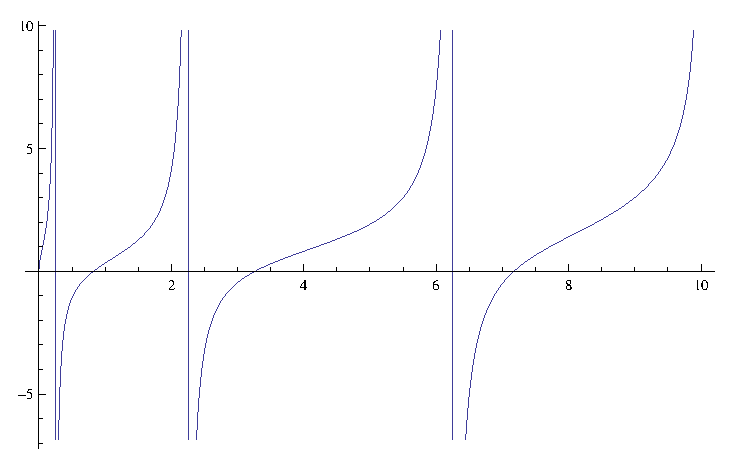
\includegraphics[scale=1.0]{Prob3.partc.eps}
\end{center}
We see from this plot that the zero crossing are the energy states and we find that $E_1 = 0.8305\widetilde{E}$, $E_2 = 3.261\widetilde{E}$, and $E_3 = 7.165\widetilde{E}$.
\item
Since we are saying that our given energies are $\sqrt{E/\widetilde{E}}$ goes like the infinite square well so we can say that 
$$\sqrt{\frac{E}{\widetilde{E}}} = n$$

\item
Now that we have the wavefunction
$$\psi(x) = \left\{\begin{array}{ll}
	B\sin(kx)	&0<x<a\\
	Ce^{-\kappa x}	&x>a
	\end{array}\right.$$
We can normalize this wavefunction
\begin{align*}
1 &= \int_{-\infty}^{\infty}\psi^*\psi dx\\
&= \int_{0}^{a}|B|^2\sin^2(kx)dx+\int_a^{\infty}|C|^2e^{-2\kappa x}dx\\
&= |B|^2\int_{0}^{a}\frac{1}{2}-\frac{1}{2}\cos(2kx)dx+\int_a^{\infty}|C|^2e^{-2\kappa x}\\
&= |B|^2\left(\frac{1}{2}x-\frac{1}{4k}\sin(2kx)\right|_0^a+|C|^2\left(-\frac{1}{2\kappa}e^{-2\kappa x}\right|_a^{\infty}\\
&= |B|^2\left(\frac{a}{2}-\frac{1}{4k}\sin(2ka)\right)-\frac{|C|^2}{2\kappa}\left(0-e^{-2\kappa a}\right)\\
&= |B|^2\left(\frac{a}{2}-\frac{1}{4k}\sin(2ka)\right)+\frac{|C|^2}{2\kappa}e^{-2\kappa a}
\end{align*}
So we still have 2 unknowns, but if we apply the boundary condition at $x=a$ we get
\begin{align*}
\psi_I(a) &= \psi_{II}(a)\\
B\sin(ka) &= Ce^{-\kappa a}\\
B &= C\frac{e^{-\kappa a}}{\sin(ka)}
\end{align*}
So if we replace $B$ in terms of $C$ we get
\begin{align*}
1 &= |B|^2\left(\frac{a}{2}-\frac{1}{4k}\sin(2ka)\right)+\frac{|C|^2}{2\kappa}e^{-2\kappa a}\\
1 &= |C|^2\frac{e^{-2\kappa a}}{\sin^2(ka)}\left(\frac{a}{2}-\frac{1}{4k}\sin(2ka)\right)+\frac{|C|^2}{2\kappa}e^{-2\kappa a}\\
1 &= |C|^2e^{-2\kappa a}\left(\frac{a}{2\sin^2(ka)}-\frac{1}{4k}\frac{2\sin(ka)\cos(ka)}{\sin^2(ka)}+\frac{1}{2\kappa}\right)\\
1 &= |C|^2e^{-2\kappa a}\left(\frac{a}{2\sin^2(ka)}-\frac{1}{2k}\cot(ka)+\frac{1}{2\kappa}\right)\\
|C| &= e^{\kappa a}\left(\frac{a}{2\sin^2(ka)}-\frac{1}{2k}\cot(ka)+\frac{1}{2\kappa}\right)^{-1/2}\\
\end{align*}
And we can say that $B$ is
\begin{align*}
B &= C\frac{e^{-\kappa a}}{\sin(ka)}\\
&= \frac{e^{-\kappa a}}{\sin(ka)}e^{\kappa a}\left(\frac{a}{2\sin^2(ka)}-\frac{1}{2k}\cot(ka)+\frac{1}{2\kappa}\right)^{-1/2}\\
&= \frac{1}{\sin(ka)}\left(\frac{a}{2\sin^2(ka)}-\frac{1}{2k}\cot(ka)+\frac{1}{2\kappa}\right)^{-1/2}
\end{align*}
Assuming $a=10$ and $m=0.01$ we can see the plots of the first two energy states
\begin{center}
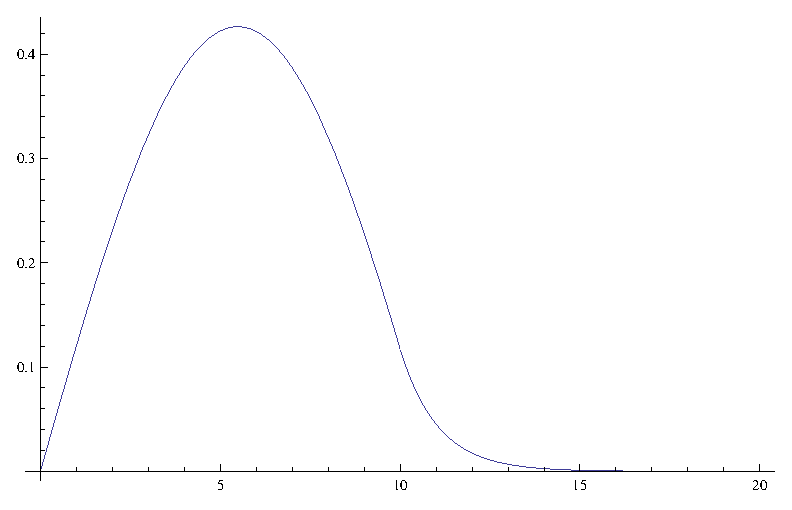
\includegraphics[scale=0.75]{Prob3.partd.eps}
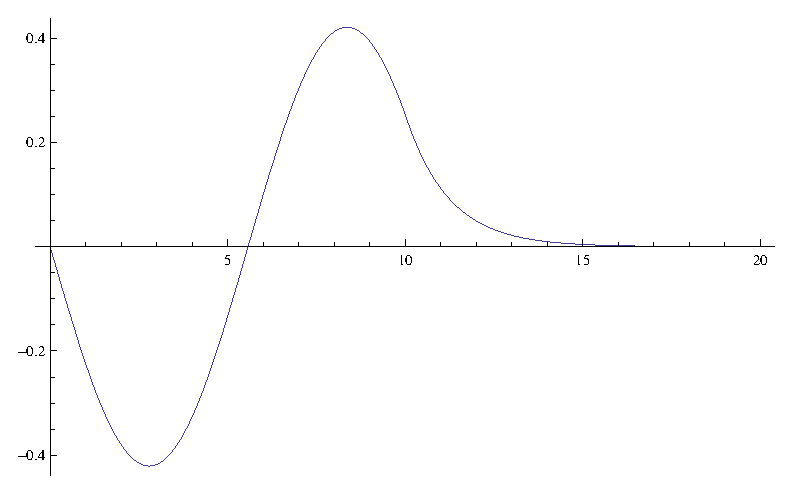
\includegraphics[scale=0.75]{Prob3.partd2.eps}
\end{center}

\end{enumerate}

\section{Problem \#4}
\begin{enumerate}[(a)]
\item
Since we have no potential in this system we can say that the solution to equation \ref{TISE} is
$$\psi(x) = Ae^{ikx}+Be^{-ikx}$$
Now we need to apply the boundary condition that $\psi(x) = \psi(x+L)$. So
\begin{align*}
Ae^{ikx}+Be^{-ikx} &= Ae^{ik(x+L)}+Be^{-ik(x+L)} \\ 
Ae^{ikx}+Be^{-ikx} &= Ae^{ikx}e^{ikL}+Be^{-ikx}e^{-ikL}
\end{align*}
Now we see that for this to be true we need
$$e^{-ikL} = e^{ikL} = 1$$
to be true. This implies that $kL = 2n\pi$ so we see that 
$$k = \frac{2n\pi}{L}$$
So to normalize the function we normalize the two functions separately since the particle can't be going in both directions.
\begin{align*}
1 &= \int_{-\infty}^{\infty} \psi^*\psi dx\\
&= \int_{0}^{L}Ae^{-ikx}Ae^{ikx}dx\\
&= \left.A^2x\right|_0^L\\
&= A^2L\\
A &= \frac{1}{\sqrt{L}}
\end{align*}
And we see for the opposite direction we get
$$B = \frac{1}{\sqrt{L}}$$
So our wave function is
$$\psi(x) = \frac{1}{\sqrt{L}}e^{ikx}+\frac{1}{\sqrt{L}}e^{-ikx}$$
where 
$$k = \frac{2n\pi}{L}$$

\item
If we were to write this in terms of $\varphi$ we see that $x$ is like the arc length. So we can relate $\varphi$ to $x$ by using the arch length formula
$$x = R\varphi$$
where $R$ is our radius which in terms of $L$ is 
$$R = \frac{L}{2\pi}$$
So we can say that
$$x = \frac{L}{2\pi}\varphi$$

\item
The two degenerate states are the two directions the particle can be traveling anti-clockwise and clockwise. If we wanted to make an eigenstate operator where each direction is different we can say 
$$\hat{L} = \frac{\partial}{\partial\varphi}$$
see that each direction is different by a negative.
\end{enumerate}
\end{document}

